\documentclass[11pt]{article}
\usepackage{hyperref}
\usepackage{amsmath, amsfonts, amssymb, mathrsfs, dsfont}
\usepackage{dcolumn}
\usepackage{caption}
\usepackage{subcaption}
\usepackage{filemod}
\usepackage{natbib}
\usepackage[ruled, vlined]{algorithm2e}
\usepackage{floatrow}
\usepackage{setspace}
\usepackage{verbatim}
\usepackage{graphicx}

\hypersetup{
    colorlinks=true,
    linkcolor=blue, 
    urlcolor=black,
    citecolor=blue, 
    }

\oddsidemargin=0.25in
\evensidemargin=0.25in
\textwidth=7in
\textheight=8.75in
\topmargin=-.5in
\addtolength{\oddsidemargin}{-.5in}
\addtolength{\evensidemargin}{-.5in}
\footskip=0.5in
\doublespacing

\title{Deep Gaussian Processes and Hierarchical Modeling with Functional Data: A Case Study in Cosmological Power Spectra}
\author{Stephen A. Walsh\thanks{Corresponding author: Division of Natural Sciences, 
        Math and Technology, Elms College, {\tt walshst@elms.edu}} \and 
        Annie S. Booth\thanks{Department of Statistics, North Carolina State University} \and
        David Higdon\thanks{Department of Statistics, Virginia Tech} \and
        Marco A.R. Ferreira\footnotemark[3] \and
        Kelly Moran\thanks{Los Alamos National Laboratory} \and
        Katrin Heitmann\thanks{Argonne National Laboratory}}
\date{\today}


\begin{document}

\maketitle
\bigskip

\begin{abstract} 
Understanding the structure of our universe and how matter is spread out and expanding is an area of active research. As cosmological surveys grow in complexity, developing surrogate models to efficiently predict matter power spectra is an important research area in cosmology. In this work, we synthesize methods from deep Gaussian processes, Bayesian hierarchical modeling, and basis functions in a novel way to estimate and predict matter power spectra (which are functional in nature) for different cosmologies. Our method has favorable results compared to the benchmark cosmological emulator (Cosmic Emu), and our code is available in a repository.
\end{abstract}

%\vfill

\section{Introduction}
%%%%%%%%%%%%%%%%%%%%%%%%%%%%%%%%%%%%%%%%%%%%%%%%%%%%%%%%%%%%%%%%%%%%%%%%%%%%%%%

To further our understanding of the structure and movement of the universe, researchers utilize numerous cosmological surveys such as the Sloan Digital Sky Survey \citep{york2000sloan} and the upcoming Nancy Grace Roman Space Telescope \citep{Dore2019WFIRST} which are continuously growing in complexity. With these tools, cosmologists aim to continue learning more about cosmic acceleration \citep{caldwell2009physics}. To this end, one important ingredient to aid in this understanding of our universe is the matter power spectrum. 

The matter power spectrum is a fundamental concept in cosmology and describes the distribution of matter as a function of spatial scale. It is often represented as a function of wavenumber $k$ (units Mpc$^{-1}$), which is inversely related to spatial scale. On large scales (i.e., small $k$ values), cosmic expansion dynamics and the matter power spectrum behave according to linear perturbation theory \citep{pietroni2008flowing, lesgourgues2009non}. On smaller scales, non-linear dynamics require the use of computationally intensive simulations; the Coyote Universe \citep{lawrence2010coyote} and more recently the Mira-Titan Universe \citep{moran2023mira} are two simulation suites dedicated to this effort. 

Leveraging these simulations allows for emulation and prediction of the matter power spectrum under varying specifications for eight different cosmological parameters (i.e., different cosmologies). Estimating and understanding the influence of these parameters on cosmic expansion are areas of active research. In addition to presenting the Mira-Titan simulation suite, \cite{moran2023mira} builds off of previous spectrum emulation \citep{lawrence2017mira} to provide the final emulator (Cosmic Emu) based on the full suite of simulations. 

In this work, we expand on the previous emulation methods and propose a novel synthesis of methods to quantify uncertainty and predict matter power spectra for different cosmologies using deep Gaussian processes (DGPs). In order to handle multiple realizations of functional output (from the Mira-Titan simulation suite), we use hierarchical and basis functions modeling within our DGP framework to accurately estimate and predict power spectra for different cosmologies. When comparing to Cosmic Emu, we see favorable results for our method. The code to reproduce these results are available at \url{https://github.com/stevewalsh124/dgp.hm}. \textcolor{red}{Please note: this repository is currently private until we hear back regarding permissions for sharing the Mira-Titan data alongside our code.}

The remainder of the paper is organized as follows: Section \ref{sec:data} provides more details regarding the Mira-Titan simulation suite. Section \ref{sec:hm_fit} describes our model and the training procedure for both toy data as well as the Mira-Titan dataset. With this trained model, Section \ref{sec:pred} explains our modeling approach for predictions at held-out cosmologies and compares with other methods. Section \ref{sec:disc} concludes with a discussion of our contributions and avenues for future research.

\section{Data}
\label{sec:data}

The Mira-Titan simulation suite is a dataset consisting of simulated power spectra for 117 different cosmologies. Each of these cosmologies is specified by 8 cosmological parameter values, which we will denote as $\theta \in \mathbb{R}^8$. Different simulation output exists for different values of a ninth value, the redshift; in this work, we fix this value at 0. For each cosmology, we have a set of 18 simulated spectra: an inexpensive spectrum estimated from linear perturbation theory ($y_p$), 16 spectra estimated from lower-resolutions simulations ($y_{\ell_r}, r \in \{1,\dots,16\}$), and one spectrum from a high resolution simulation ($y_h$). 

These spectra are represented as a function of wavenumber $k$, and hence is denoted $P(k)$. Following \cite{moran2023mira}, we model on the emulation space $\mathcal{P}(k)=\log_{10}\left(\frac{k^{1.5}P(k)}{2\pi^2}\right)$. The output is available for $0.001 \leq k \leq 5$ for $n=351$ different values of $k$, but each data type has differing values where it is deemed approximately unbiased. For $k<0.04$, only $y_p$ provides a reliable estimate of the spectra. $y_{\ell_r}$ are valid for $0.04 \leq k \leq 0.25$, and $y_h$ is valid for $0.04 \leq k \leq 5$. Figure \ref{fig:plot_data} shows an example of the output for a particular cosmology.

\begin{figure}[ht]
    \centering
    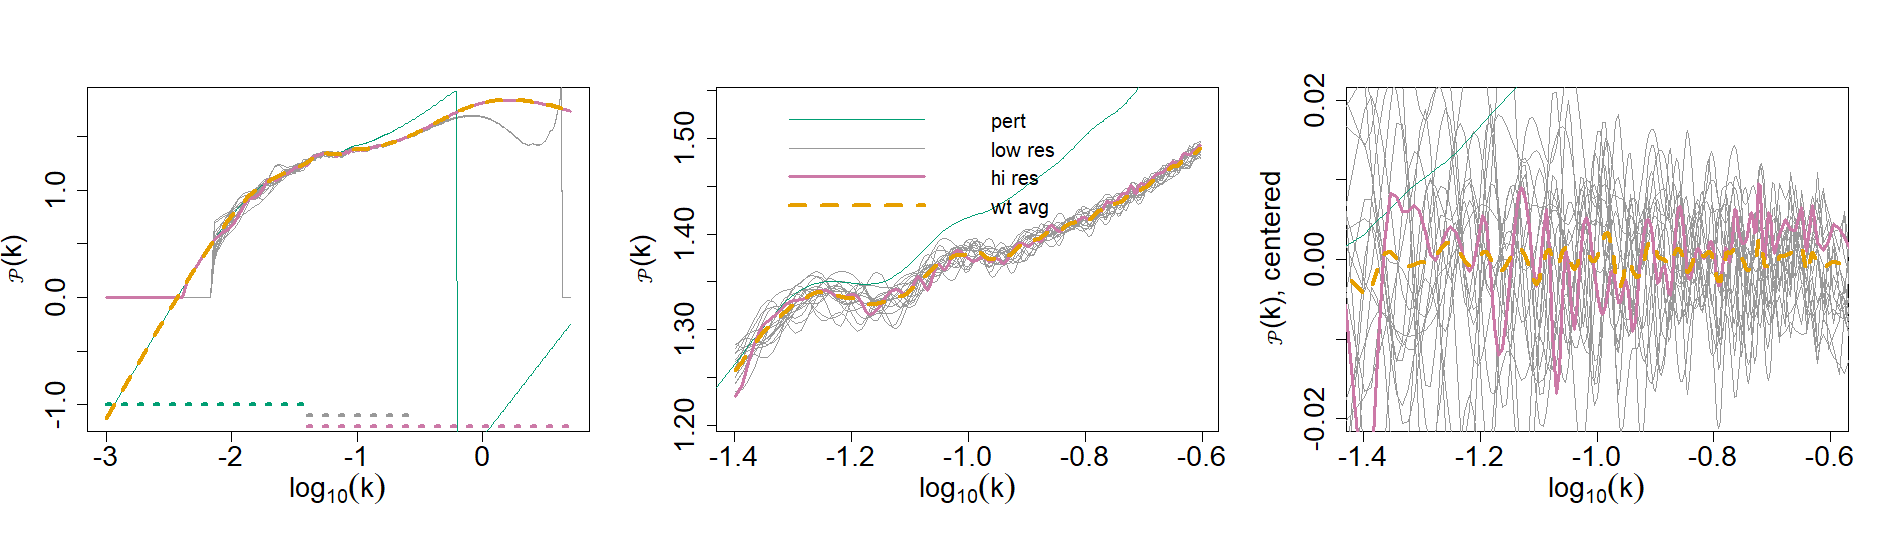
\includegraphics[width=6in]{plot_data.png}
    \caption{Left: The perturbation theory, low resolution runs, and high resolution run for the first training cosmology. The weighted average is also shown as a dashed line. Dotted lines at the bottom indicate where each data type is deemed approximately unbiased. Right: The same image, but only where the low resolution runs are approximately unbiased.}
    \label{fig:plot_data}
\end{figure}

From the multiple low- and high-resolution spectra across all cosmologies, \cite{moran2023mira} obtained estimates for the precision of these spectra across the $n$ wavenumber values ($p_1,\dots,p_n$) using a log-log regression model, and a multiplier $c$ for the increase in precision from the low- to high- resolution output. Given that the perturbation theory spectra is non-stochastic, we treat this as having a precision of $10^5$. We leverage these precision estimates within our model at each data type's unbiased wavenumber values to define $\Lambda_p = \text{diag}\left((10^5)_{k < 0.04}\right)$, $\Lambda_{\ell} = \text{diag}\left(16(p_1,\dots,p_n)_{0.04 \leq k < 0.25}\right)$, $\Lambda_h = \text{diag}\left(c(p_1,\dots,p_n)_{0.04 \leq k \leq 5}\right)$. Here, each precision matrix is diagonal and the diagonal elements consists of the precision values or zero, depending on whether the $k$ value is approximately unbiased for that data type. With this, we calculate a weighted average for each cosmology: $\bar y = \Lambda^{-1}(\Lambda_p y_p + \Lambda_h y_h + \Lambda_{\ell} \bar{y}_\ell)$, where $\Lambda = \Lambda_p + \Lambda_\ell + \Lambda_h$ is the precision matrix for the weighted average for a particular cosmology.

We will handle the data in two stages.  First, we will focus on 111 training cosmologies and obtain the best esimated spectrum for each.  Second, we will use these estimates to predict the spectra for six held-out cosmologies.

\section{Bayesian Hierarchical Modeling for Particular Cosmologies}
\label{sec:hm_fit}

Here we describe our first contribution: the use of a Bayesian hierarchical model to estimate the underlying spectra (and quantify uncertainty) for a particular cosmology.  We focus solely on one cosmology, independent of the others.

\subsection{Gaussian Process Model}

Here, we introduce the Bayesian Gaussian Process (GP) model leveraging the aggregated data $D_n \equiv \{X_n, \bar Y, \Lambda\}$ for a particular cosmology. We assume the matter power spectrum $S$ for a given cosmology follows a GP with mean $\mu$ and covariance matrix $\Sigma_S$.

From plots of the multiple low-resolution spectra, we find they vary smoothly about some mean $S$, suggesting that a dense covariance matrix $\Sigma_\varepsilon$ may outperform a diagonal covariance $\Lambda_\ell^{-1}$ for $\bar Y$. In previous work, we have modeled multiple candidates for $\Sigma_\varepsilon$ \citep{walsh2023bayesian} and found that a Mat\'ern covariance $\Sigma_\ell$ trained on the low-resolution runs (pre-scaled by the precision values and subtracting a LOESS-smoothed average) performs the best. We specify this structure within $\Sigma_\varepsilon$ and refer readers to \cite{walsh2023bayesian} for a more detailed exposition. This yields $\Sigma_\varepsilon=\left(\Lambda_p^{-1} + \Sigma_\ell + \Lambda_h^{-1}\right)^{-1}$, where $\Lambda_p, \Sigma_\ell^{-1}, \text{ and } \Lambda_h$ are all $n\times n$ and are 0 wherever the corresponding data type is biased.

We transform $X$ values to fall within $[0,1]$ and $Y$ so that the mean and variance are 0 and 1, respectively. This allows for a strightforward specification of priors, where the hyperparameters for each Mat\'ern covariance $\Sigma_S$ and $\Sigma_\ell$ each take a vague inverse-Gamma prior. Specifically:

\begin{align}
\Sigma_\ell^{i,j} = \tau_\ell^2  \left( 1 + \frac{\sqrt{5}d}{\sqrt{\theta_\ell}} + \frac{5d^2}{3\theta_\ell}\right) \exp\left(-\frac{\sqrt{5}d}{\sqrt{\theta_\ell}}\right),\\
\Sigma_S^{i,j} = \tau_S^2  \left( 1 + \frac{\sqrt{5}d}{\sqrt{\theta_S}} + \frac{5d^2}{3\theta_S}\right) \exp\left(-\frac{\sqrt{5}d}{\sqrt{\theta_S}}\right),
\end{align}

where $d=||x_i-x_j||^2$. From here, we estimate $\tau_\ell, \theta_\ell$ with maximum likelihood, and conditional on $\Sigma_\varepsilon$, we specify priors for $\tau_S, \theta_S$ following \cite{sauer2023active}:

\textcolor{cyan}{Annie, please put the newest prior specs here.}

% $$
% \mathbf{\Sigma_\varepsilon} =
% \begin{bmatrix}
% \Lambda_p^{-1} & \mathbf{0} & \mathbf{0} \\
% \mathbf{0} & \mathbf{\Sigma}_{\ell} & \mathbf{0} \\
% \mathbf{0} & \mathbf{0} & \Lambda_h^{-1}
% \end{bmatrix}
% $$

Therefore, we model $\bar Y|S$ as a GP with mean $S$ and block-diagonal covariance matrix $\Sigma_\varepsilon$:

\begin{align}
\bar Y|S &\sim \mathcal{N}_n(S,\Sigma_\varepsilon) \\
S &\sim GP\left(\mu, \Sigma_S(x,x')\right)
\end{align}

Upon integrating out $S$, we obtain $\bar Y \sim GP(\mu, \Sigma_S+\Sigma_\varepsilon)$. Additionally, this model yields the posterior distribution $S|\bar Y \sim N(m, C)$, where $C=\left(\Sigma_S^{-1}+\Sigma_\varepsilon^{-1}\right)^{-1}$ and $m=C\left(\Sigma_\varepsilon^{-1}\bar Y+\Sigma_S^{-1}\mu\right)$. 

This distribution provides the posterior mean and corresponding uncertainty for $S$ within a given cosmology. Without this hierarchy, uncertainty would not be properly addressed; the weighted average would simply be nearly interpolated across the relatively dense set of $k$ values.

\subsection{Deep Gaussian Process Model}

Considering the Mira-Titan data, some nonstationarity is expected (e.g., due to baryonic acoustic oscillations when $-2 \leq \log_{10}(k) \leq -1$). To account for this, we incorporate a latent layer warping $W$ within the hierarchical model to incorporate nonstationary dynamics of the matter power spectra. When $W$ is a GP, this creates a deep Gaussian process (DGP) model \citep{damianou2013deep}. Additional latent layers could be considered, although one is sufficient for this dataset \citep{dunlop2018deep}.


\begin{align}
\bar Y|S,W &\sim \mathcal{N}_n(S,\Sigma_\varepsilon) \\
S|W &\sim GP\left(\mu, \Sigma_S(w,w')\right) \\
W &\sim GP\left(0, \Sigma_W(x,x')\right)
\end{align}

We have found that whether the prior mean of $W$ is set to 0 or $X$ \citep[which would indicate stationarity apriori, ][]{schmidt2003bayesian} does not have a substantial impact on the model fit. We construct this model in the compositional form, and also use MCMC to obtain full uncertainty for each of the model parameters \citep{sauer2023active}.

\textcolor{cyan}{Annie: want to add something here? We discuss the elliptical slice sampling of $W$, but otherwise it is plugged in to the methods of the previous section with very few changes.}

Through the synthesis of the DGP model alongside the additional level of hierarchical modeling (HM) to incorporate multiple functional model runs, we call this method DGP.HM.

\subsection{Simulation Study}
\label{subsec:sim}

We compare our DGP.HM model to competing models with a simulation study, in which case the true curve is known. Following \cite{moran2024dpc}, we consider two functions ($f_1$ and $f_2$) each with two variance specifications (settings ``4" and ``5", \textcolor{magenta}{we can consider additional homoskedastic cases in the appendix if necessary}). 

Here, $f_1$ and $f_2$ are defined as follows:

\begin{align}
  f_1(x) &= m_1 \exp(-u_1x/2) * \cos(wx) - m_1x/5, \quad w=\sqrt{25-[u_1/2]^2} \\
  f_2(x) &= \exp(-m_2[x-3]^2)+\exp(-u_2[x-1]^2)-0.05\sin(8[x-1.9]), \\ 
  \quad x &\in [0,4].
\end{align}

For additional variation, the values of $m_1, m_2, u_1,$ and $u_2$ are random variables where $m_1 \sim \text{Uniform}(0.5,1.5)$, $u_1 \sim \text{Uniform}(1.5,2.5)$, and $m_2,u_2 \sim \text{Uniform}(0.6,1.4)$. For each simulated function and variance specification, we generate 20 values of $m_1, m_2, f_1, f_2$, and conditional on these values, we sample either 5 or 20 functional observations and estimate the underlying true function based on the observations.

\begin{figure}[h]
    \centering
    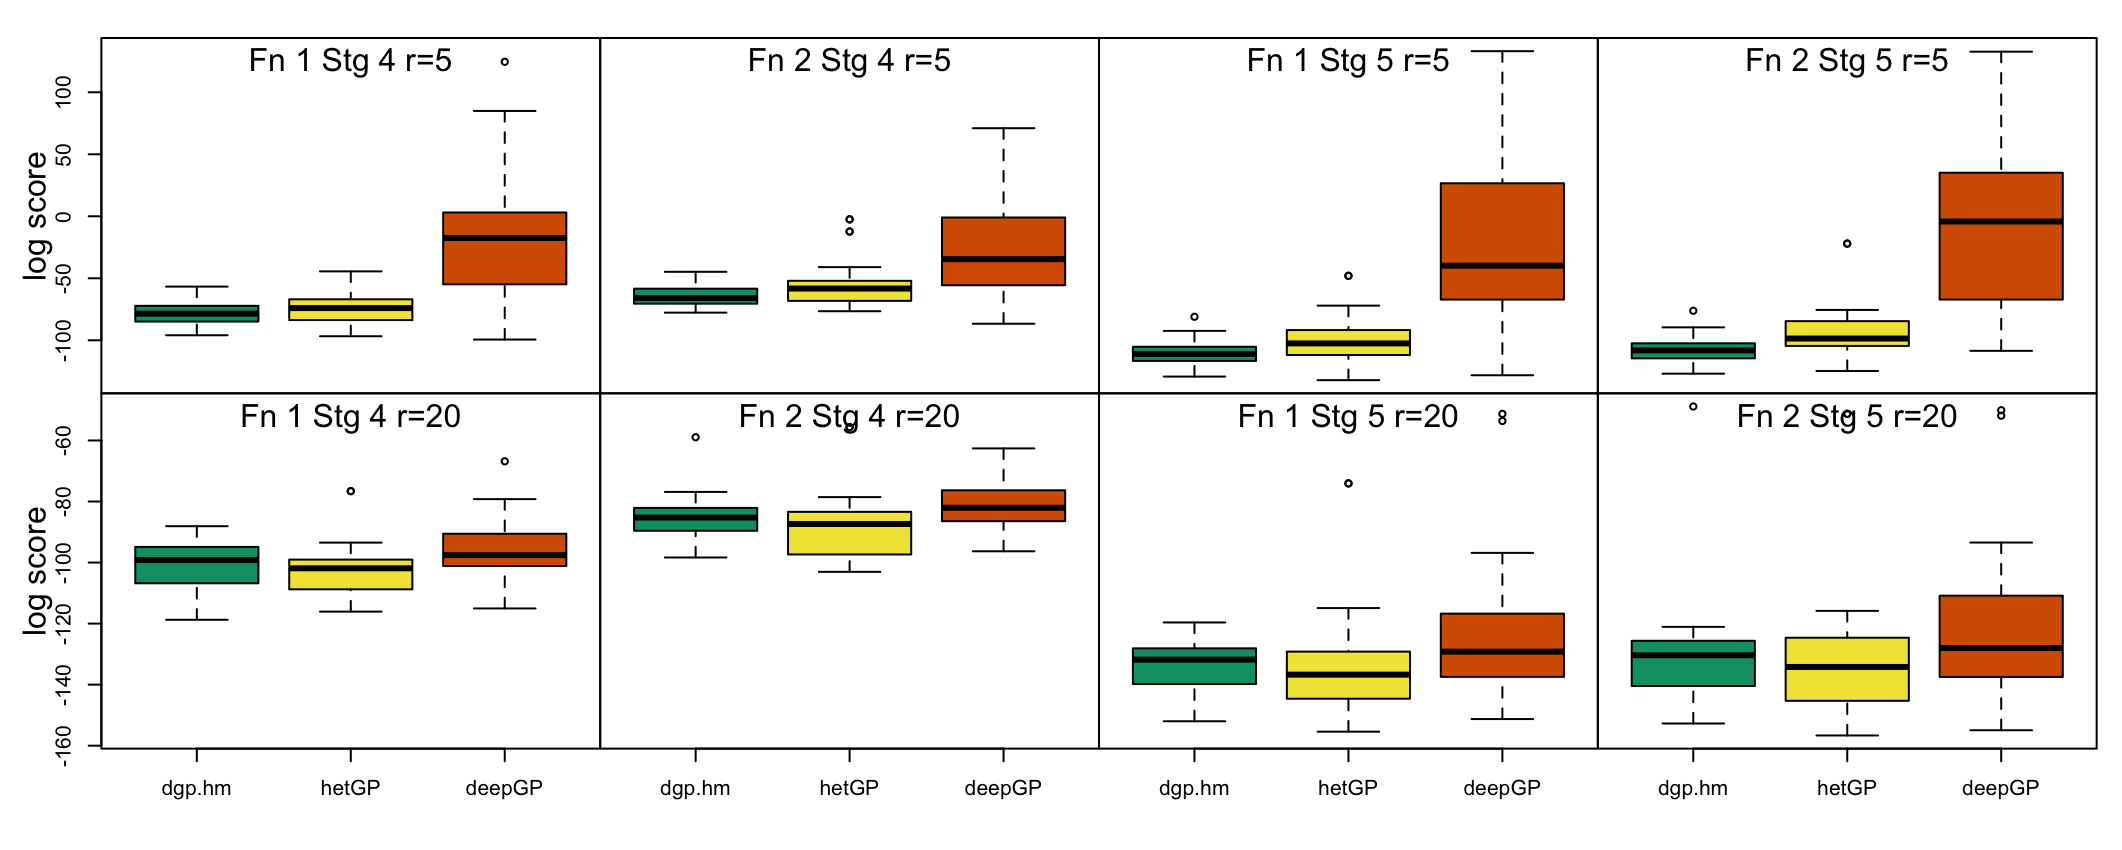
\includegraphics[width=6in]{sims_logS.png}
    \caption{Boxplot of log scores across two different functions and covariance settings (lower is better). For each case, the boxplot is constructed from 20 random batches were simulated. Each column represents a function/variance specification pair, and each row shows results for batch sizes of either 5 (top) or 20 (bottom).}
    \label{fig:sims_logS}
\end{figure}

The competing methods we consider are an out-of-the-box DGP fit using the \texttt{deepgp} package \citep{sauer2023active}, a heteroskedastic GP fit using the \texttt{hetGP} package \citep{binois2018practical, binois2021hetgp}, as well as a deep process convolution (DPC) approach, which is utilized within Cosmic Emu \citep{moran2023mira}. 

The metrics we use to evaluate performance are mean squared error (MSE) and the log score, a proper scoring rule which takes both prediction and intervals into consideration \citep{gneiting2007strictly}. For both metrics, a lower value indicates better performance. MSE and log score results are shown in Figures \ref{fig:sims_MSE} and \ref{fig:sims_logS} respectively; our DGP.HM model performs favorably against these current benchmark methods.

\begin{figure}
    \centering
    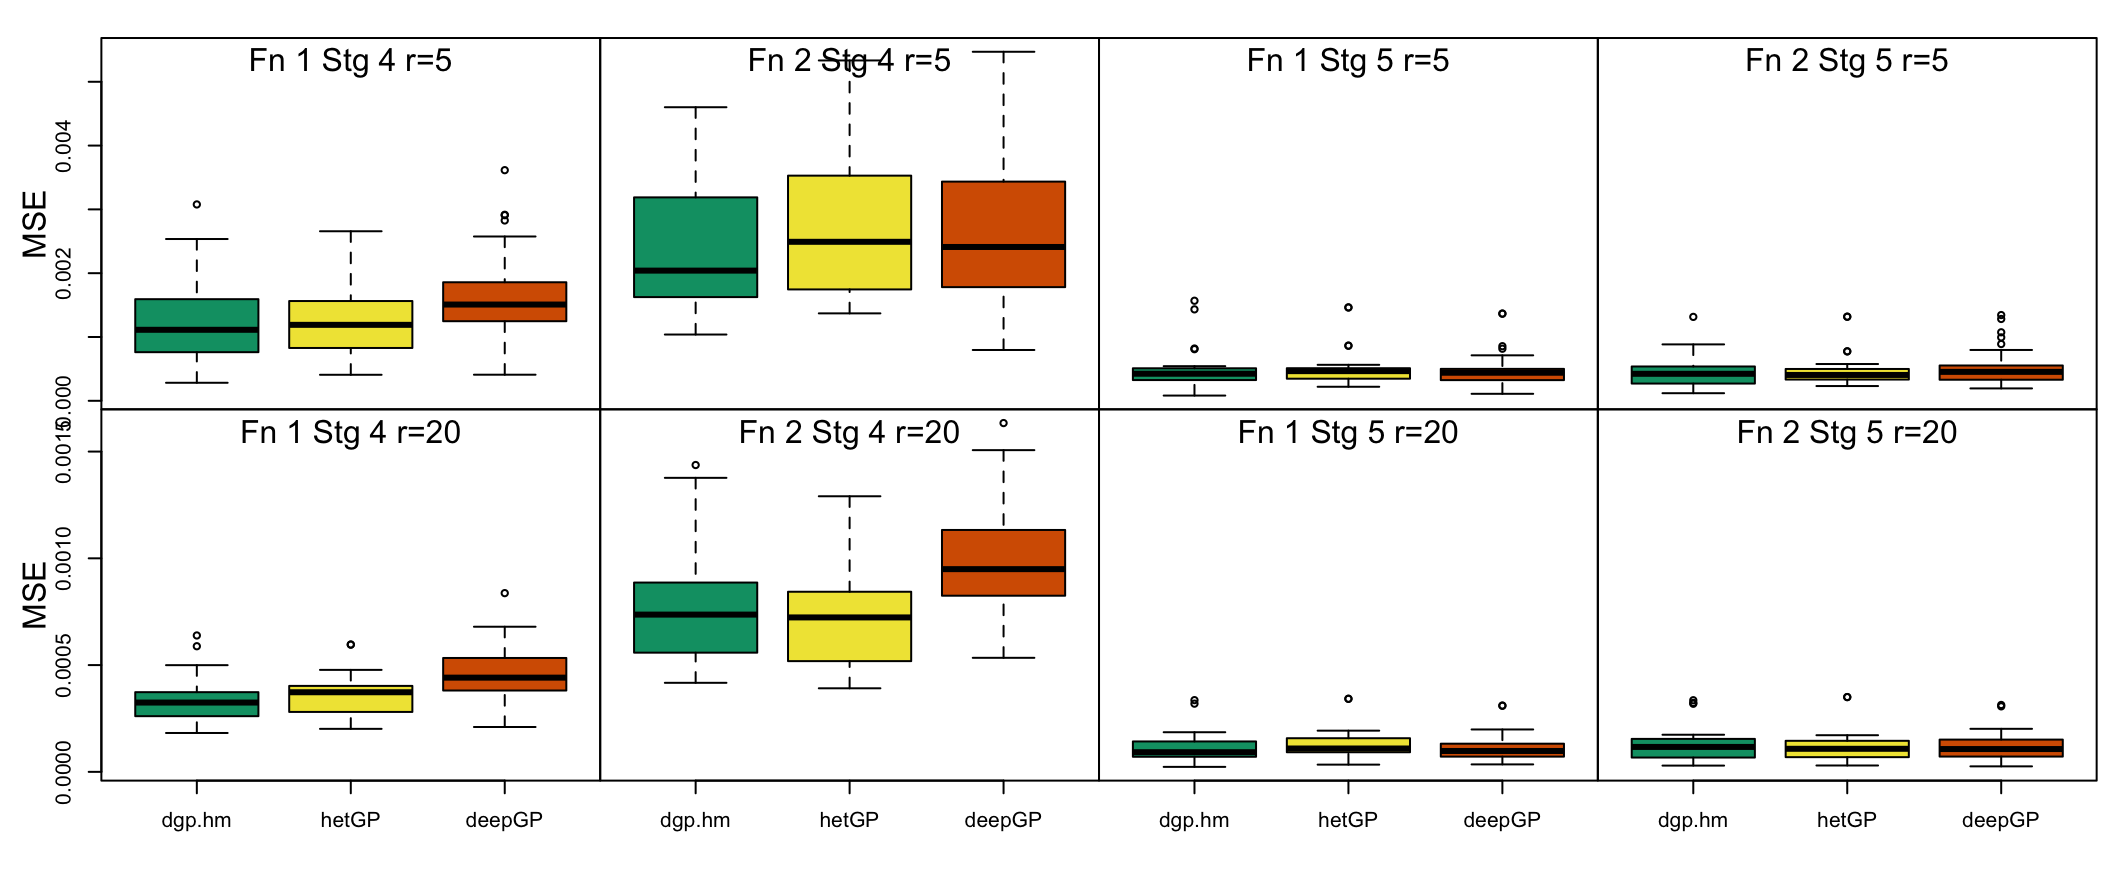
\includegraphics[width=6in]{sims_MSE.png}
    \caption{Boxplot of MSEs across two different functions and covariance settings (lower is better). For each case, the boxplot is constructed from 20 random batches were simulated. Each column represents a function/variance specification pair, and each row shows results for batch sizes of either 5 (top) or 20 (bottom).}    
    \label{fig:sims_MSE}
\end{figure}

\subsection{CAMB Data}
\label{subsec:camb}

In addition to simulated data, we investigate model fits the for different cosmological datasets (based on linear theory and/or runs from the Code for Anisotropies in the Microwave Background, CAMB). \textcolor{magenta}{We have looked at two sets of model runs, "LT" runs where there is an underlying ``true" value alongside 15 computer model runs, or the "CAMB" runs, where we only have a single output. The performance from the CAMB runs was better (with a 6-dimensional design space), and also did not require obtaining a posterior mean from multiple model runs. When looking at the CAMB runs on the $\Delta$ space, we see it generally is withing $\pm 5\%$ error. Regarding these results, compared to the results for the 8-dimensional LT runs which had less impressive predictive performance, I'm not sure if we will include details on one or the other.}

\begin{figure}
    \centering
    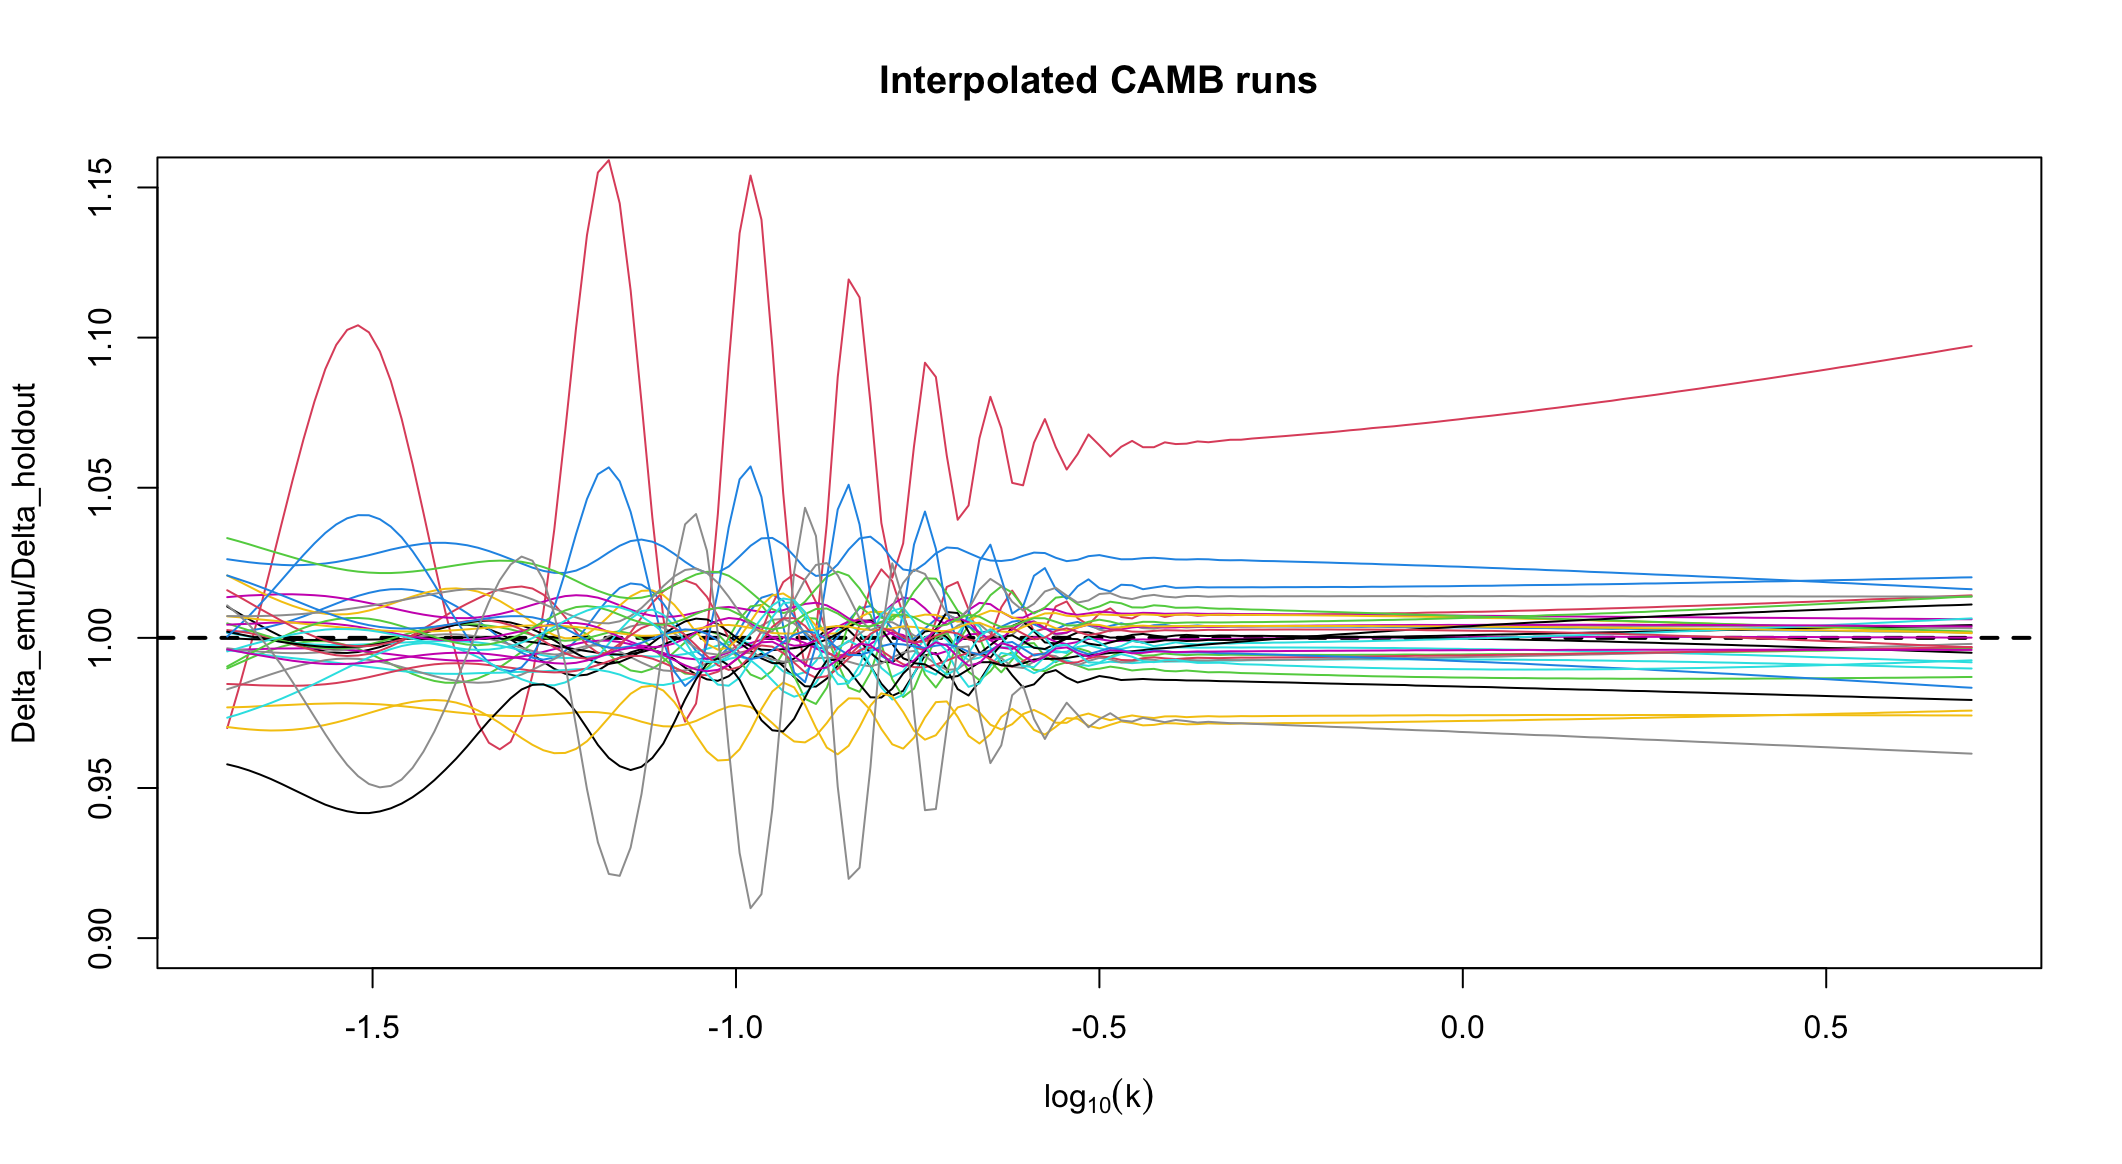
\includegraphics[width=6in]{plot_pca_CAMB.png}
    \caption{Proportion of $\Delta_{emu}$ vs. $\Delta_{holdout}$ for model runs 11-42 (excluding 27-28).}   
    \label{fig:pca_camb}
\end{figure}


\subsection{Estimating Spectra with Mira-Titan Data}
\label{subsec:mira_fit}

Estimate one cosmology with 50,000 runs, and use this as a starting point for each of the others

Here we can provide figures of the predicted mean and variances for a subset of the actual cosmologies. Figure \ref{fig:plot_fit} shows an example of the uncertainty for our posterior mean for the first (of 111) training cosmologies; the posterior mean is subtracted in order to visualize this uncertainty.

\begin{figure}[ht]
    \centering
    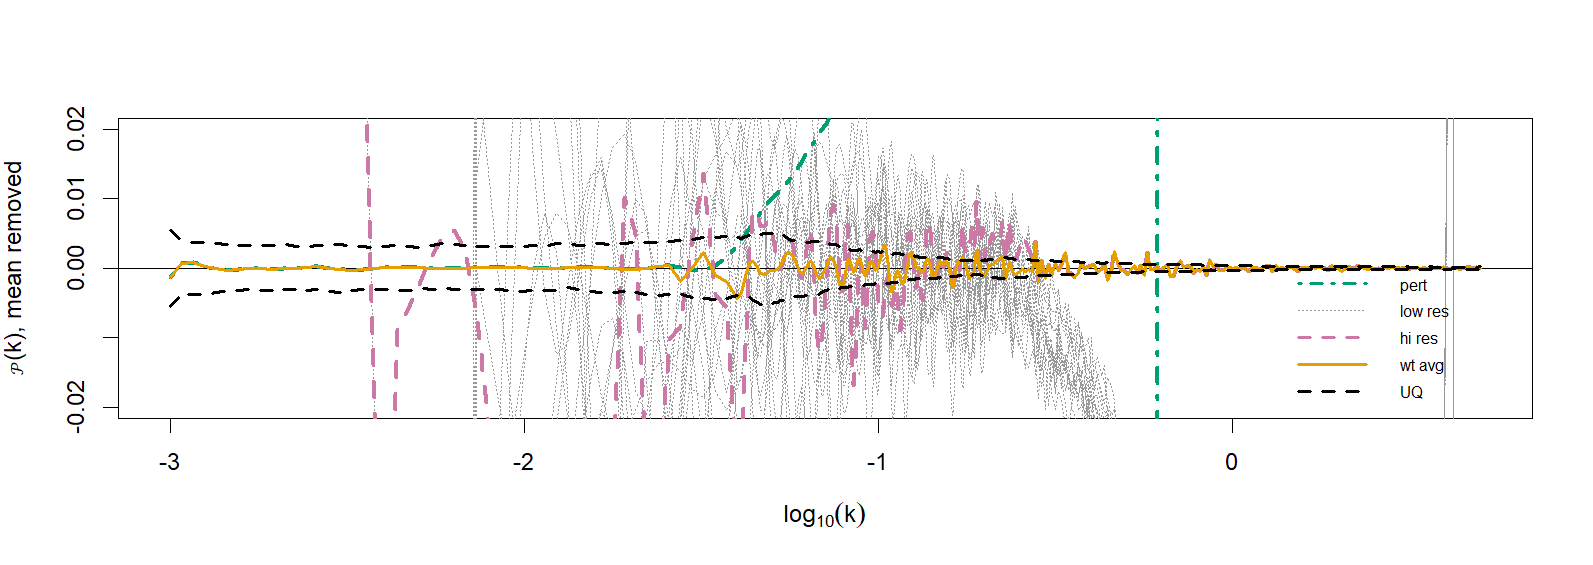
\includegraphics[width=6in]{plot_fit.png}
    \caption{95\% credible intervals for the power spectrum of model 1 (posterior mean subtracted). Plots of the perturbation theory, low-resolution and high-resolution runs are also shown, alongside the weighted average.}
    \label{fig:plot_fit}
\end{figure}

%\begin{figure}[ht]
%    \centering
%    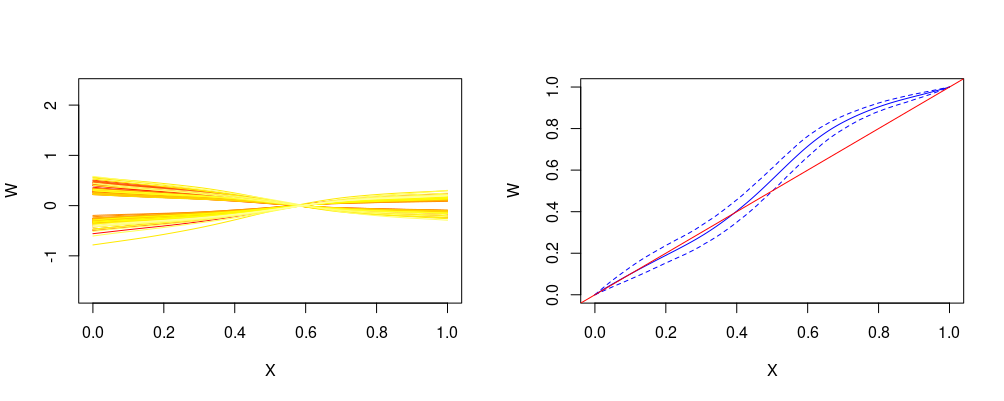
\includegraphics[width=6in]{plot_warp_M001.png}
%    \caption{Left: MCMC samples of $W$ for model M001 after burnin and thinning. Right: Corresponding 95\% credible intervals for $W$.}
%    \label{fig:plot_warp}
%\end{figure}

Images:
\begin{itemize}
    \item Illustration of DGP fit (post mean and UQ, could show cosmicEMU as well?)
    \item estimated warping (or, how all 111 warpings compare)
\end{itemize}


\section{Prediction for Unobserved Cosmologies}
\label{sec:pred}

This section details our second contribution - the use of the Bayesian DGP model of the previous section to predict the curve for held-out cosmologies.

\subsection{PCA-GP Model}
\label{subsec:pca}

Here we describe the PCA-GP model.  We discuss how we use the predicted curves that we got previously as training data. \cite{higdon2008computer, higdon2010estcosmo}

\begin{itemize}
    \item show breakdown of estimated mean trend, basis functions/PCs, and weights of a particular PC/BF.
\end{itemize}

\subsection{Predicting Spectra from Mira-Titan Data}
\label{subsec:mira_pred}

Here we show results on held-out cosmologies.  The Cosmic Emu emulator is constructed by (process convolutions, ...). Segue to our method after and compare/contrast with Cosmic Emu. 

In addition to predicting for held-out cosmologies, we can also predict over a large uniform or full factorial design to obtain estimated main effects for each parameter in $\theta$, interactions amongst the 8 parameters, and variance decomposition. Should this be included?

\begin{figure}[ht]
    \centering
    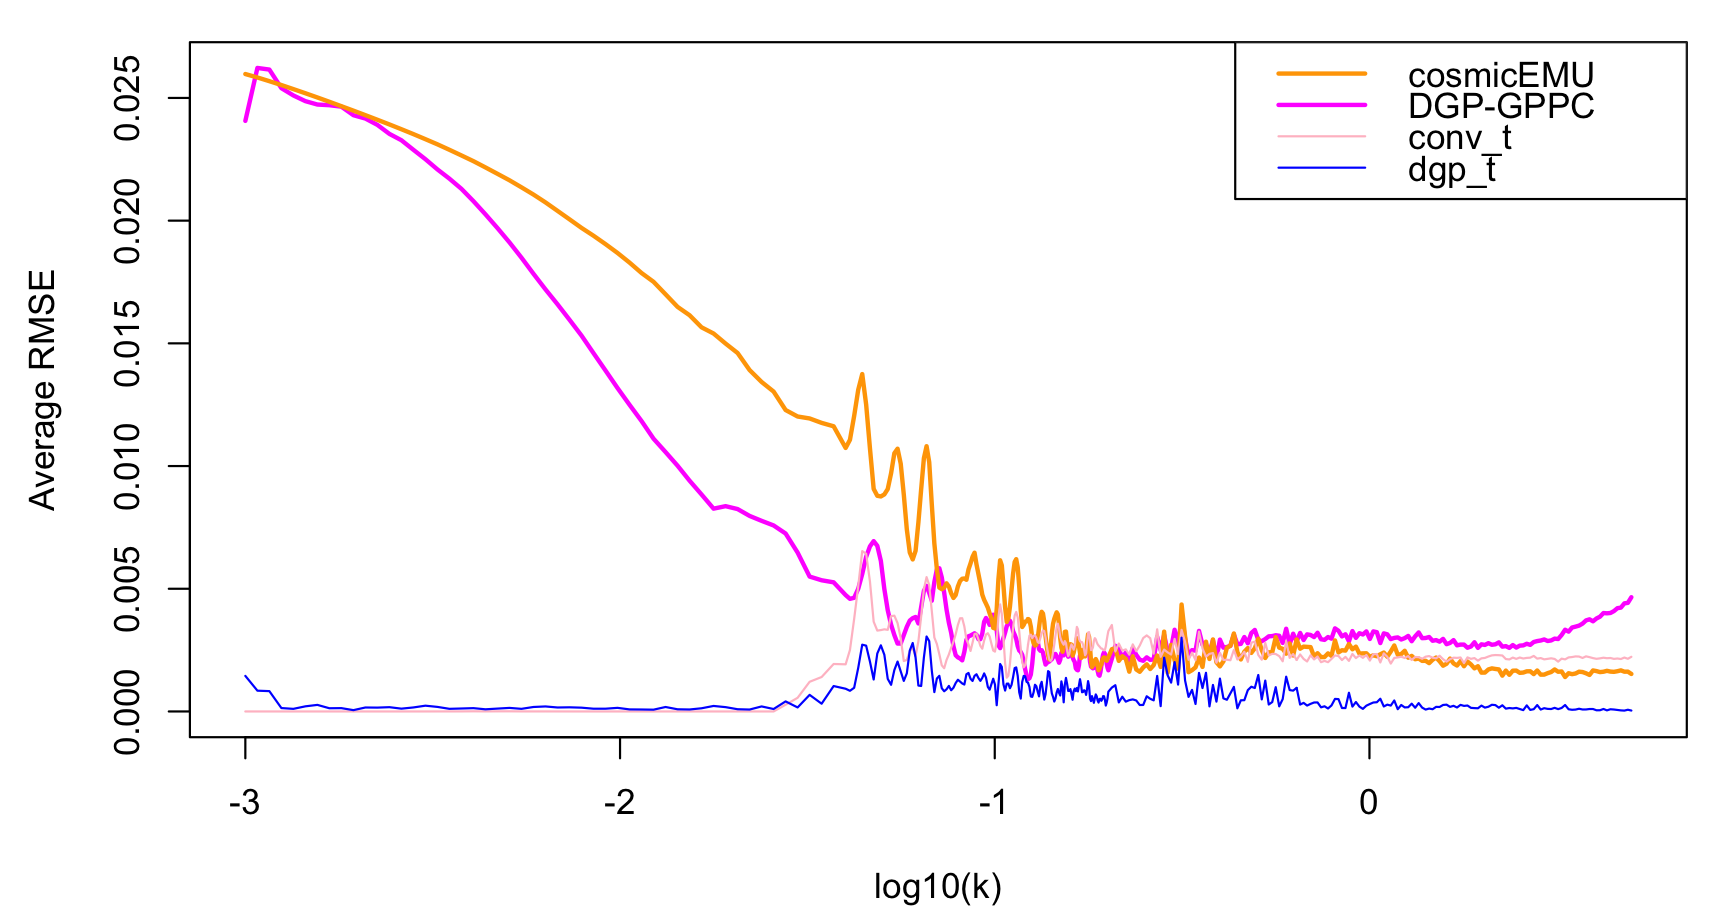
\includegraphics[width=6in]{rmse_by_k.png}
    \caption{Left: Average RMSE of each prediction method across all $k$ values. Right: Average RMSE for each method when using the held-out computer model runs to train the model. In each case, the truth is assumed to be the weighted average of the computer model runs.}
    \label{fig:plot_rmse_k}
\end{figure}

% \begin{figure}[ht]
%     \centering
%     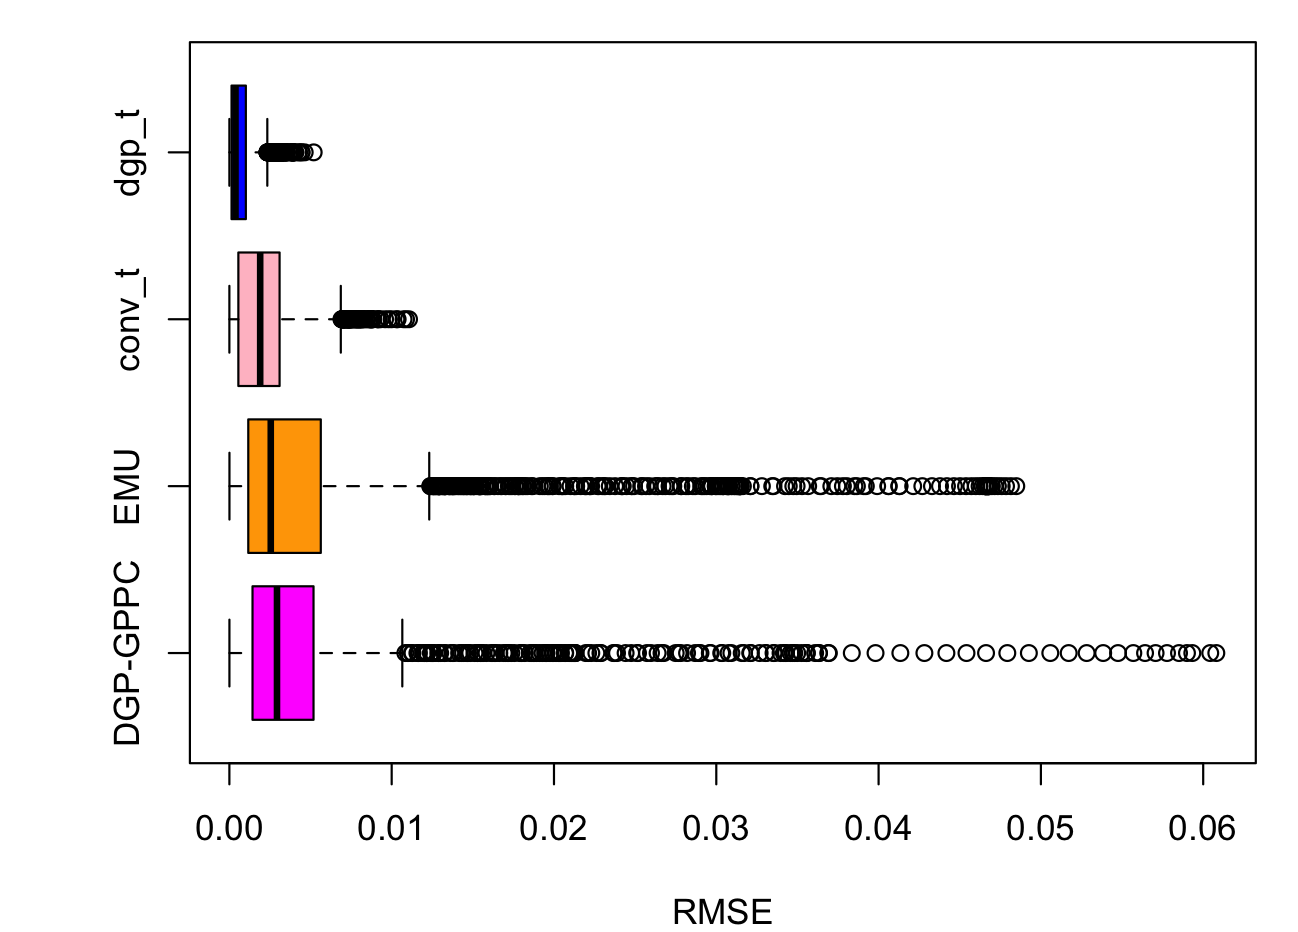
\includegraphics[width=6in]{rmse_box.png}
%     \caption{Boxplot of all RMSEs of each method across all six test models. From top to bottom: box plots for our training method, process convolution training method, Cosmic EMU predictions, and our DGP-PC predictions.}
%     \label{fig:plot_rmse_box}
% \end{figure}

\section{Discussion}
\label{sec:disc}

Brief recap, directions for future research: BSS-ANOVA in lieu of DGPs, hydrodynamical sims or TCs as other applications of this methodology. A more detailed sensitivity analysis for the parameters, modeling $W$ across different cosmologies, consider modeling for different redshift values other than $z=0$.

\section{Appendix}
\label{sec:apdx}

The different appendices from dissertation as necessary. Can also put details of dataset in supplementary material.

\begin{figure}[ht]
    \centering
    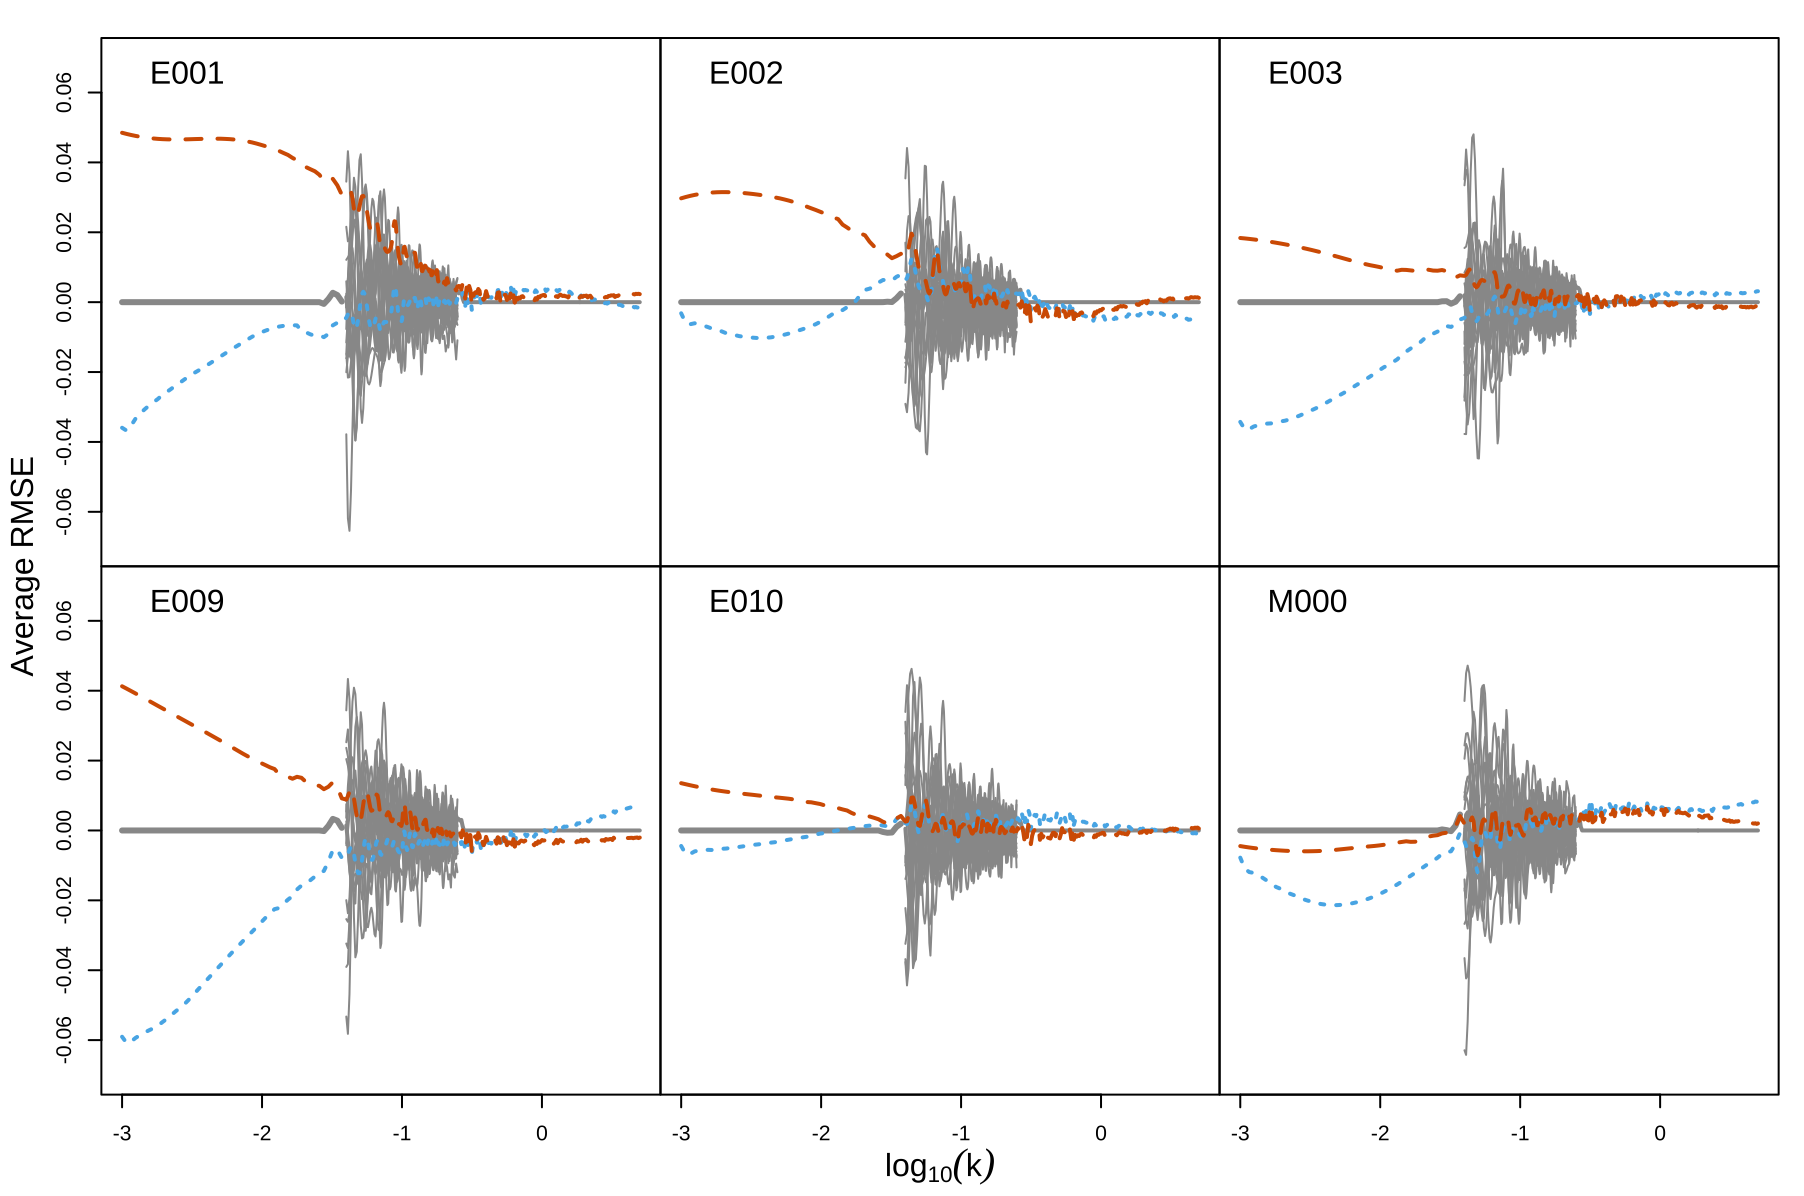
\includegraphics[width=6in]{pred_1to6.png}
    \caption{Results of all six predictions for both methods on the held-out cosmologies (weighted average subtracted). CosmicEMU is dashed, DGP.HM is dotted, and solid gray lines show results of held-out computer model runs.}
    \label{fig:plot_pred_1to6}
\end{figure}

\bibliographystyle{jasa}
\bibliography{references}

\end{document}
